\documentclass[11pt]{scrartcl}
\usepackage[pretty,polish]{mystd}
\title{Analiza}
\author{Michał Dobranowski}
\date{semestr zimowy 2022 \\ v0.0}

\begin{document}
    \maketitle
    \begin{abstract}
        Poniższy skrypt zawiera materiał obejmujący wykłady z Analizy matematycznej I oraz II prowadzone na pierwszym roku Informatyki na AGH, lecz jest mocno rozbudowany przez przykłady i twierdzenia pochodzące z przeróżnych źródeł, które (zwykle dla rozwinięcia intuicji lub ułatwienia rozwiązań pewnych zadań) postanowiłem opisać.

        PS: Analiza I nie jest skończona. Całkiem możeliwe, że nigdy nie będzie.
    \end{abstract}
    \tableofcontents
    \eject

    % \part{Analiza I}

    % Z powodu braku czasu (ale również chęci) do opisywania materiału, który -- chociaż pojawił się na wykładach -- jest, skromnym zdaniem autora, raczej szkolny, Czytelnik powinien upewnić się, że jest zaznajomiony z następującymi pojęciami: funkcja, dziedzina, przeciwdziedzina, dziedzina naturalna, injekcja, surjekcja, bijekcja, funkcja monotoniczna, (nie)rosnąca, (nie)malejąca, złożenie funkcji, funkcja odwrotna, wielomianowa, wymierna, potęgowa, wykładnicza, logarytmiczna, trygonometryczna, cyklometryczna, ciąg, podciąg.

    % \section{Granice ciągów}
    % \begin{definition}[Cauchy'ego granicy właściwej]
    \label{d:cauchy_lim_series}
    Ciąg $(a_n)$ ma granicę $g = \displaystyle\lim_{n\to\infty} a_n$ wtedy, gdy
    \[ \dforall{\eps > 0} \dexists{N \in\NN} \dforall{n\geq N} |a_n - g| < \eps. \]
\end{definition}

Jeśli ciąg $(a_n)$ ma granicę $g$, to mówimy że jest zbieżny do $g$ i piszemy $\lim a_n = g$ lub po prostu $a_n \to g$.

\begin{definition}[granicy niewłaściwej $+\infty$]
    Ciąg $(a_n)$ ma granicę niewłaściwą $\displaystyle\lim_{n\to\infty} a_n = \infty$ wtedy, gdy
    \[ \dforall{M\in\RR} \dexists{N\in\NN} \dforall{n\geq N} a_n > M. \]
\end{definition}

Analogicznie definiujemy granicę niewłaściwą w $-\infty$. Może się również zdarzyć, że ciąg nie ma granicy, na przykład $a_n = n(-1)^n$.

\begin{fact}
    Równość $\lim |a_n| = 0$ jest równoważna $\lim a_n = 0$.
\end{fact}
\begin{proof}
    Równoważność wynika z definicji \ref{d:cauchy_lim_series} i równości $\left||a|\right| = |a|$.
\end{proof}

\begin{theorem}
    \label{t:lim_subsequence=lim_sequence}
    Jeśli $\lim a_n = g$, to dla każdego podciągu $(a_{n_k})$ zachodzi $\lim a_{n_k} = g$.
\end{theorem}
\begin{proof}
    Zakładając przeciwnie, że istnieją dwa podciągi o różnych granicach, to w definicji Cauchy'ego (\ref{d:cauchy_lim_series}) wystarczy wybrać $\eps$ mniejszy niż połowa różnicy między tymi dwie granicami, aby uzyskać sprzeczność.
\end{proof}

Prosty wniosek z tego twierdzenia jest taki, że jeśli znajdziemy dwa podciągi ciągu $(a_n)$ zbiegające do różnych granic, to ciąg $(a_n)$ jest rozbieżny.

\begin{theorem}[o ciągu monotonicznym i ograniczonym]
    \label{t:sequence monotonic and bounded}
    Każdy ciąg monotoniczny i ograniczony jest zbieżny.
\end{theorem}
\begin{proof}
    Bez starty ogólności przyjmijmy, że dany ciąg $(a_n)$ jest niemalejący i ograniczony z góry przez $M = \sup\{a_n : n \in \NN\}$. Dla wszystkich $n$ zachodzi więc nierówność
    \[ a_n \leq M. \]
    Dla dowolnego $\eps > 0$ istnieje takie $a_N$, że
    \[ M - \eps < a_N \leq M, \]
    jako że w przeciwnym wypadku to $M - \eps$ byłoby supremum $(a_n)$. Skoro $(a_n)$ jest niemalejący, to dla każdego $n > N$
    \[ |M - a_n| = M - a_n \leq M - a_N < \eps, \]
    więc $\lim a_n = M$.
\end{proof}

\begin{theorem}[Bolzano-Weierstrassa]
    Jeśli ciąg jest ograniczony, to ma podciąg zbieżny.
\end{theorem}
\begin{proof}
    Udowodnimy, że jeśli z ciągu nie można wybrać podciągu niemalejącego, to można wybrać ciąg malejący, czego natychmiastowym wnioskiem (z pomocą twierdzenia \ref{t:sequence monotonic and bounded}) będzie teza.

    Najpierw zauważymy, że jeśli z ciągu nie można wybrać podciągu rosnącego, to ma on wyraz największy. Zakładając przeciwnie, mamy, że $a_1$ nie jest największy, więc szukamy większego $a_k$, który znowu nie jest największy i w ten sposób (powtarzając rozumowanie) uzyskujemy konstrukcję ciągu rosnącego. Taką konstrukcję zakłóci tylko znalezienie elementu największego.

    Załóżmy, że ciąg $(a_n)$ nie zawiera podciągu niemalejącego. Tym bardziej nie zawiera więc podciągu rosnącego, a więc ma wyraz największy, który oznaczymy $a_m$. Z ciągu $(a_{m+1}, a_{m+2}, \ldots)$ nie można wybrać podciągu niemalejącego (bo jest to podciąg ciągu $(a_n)$), więc ma on element największy, jednak mniejszy od $a_m$. Powtarzając to rozumowanie konstruujemy ciąg malejący.
\end{proof}

\begin{theorem}[o ciągu ograniczonym i ciągu zbieżnym do zera]
    \label{t:sequence bounded and convergent to 0}
    Jeśli ciag $(a_n)$ jest ograniczony oraz $\lim b_n = 0$, to
    \[ \lim_{n \to \infty} (a_n \cdot b_n) = 0 \]
\end{theorem}
\begin{proof}
    Z założenia istnieje takie $M > 0$, że dla każdego $n \in \NN$ zachodzi
    \[ -M \leq a_n \leq M. \]
    Z definicji (\ref{d:cauchy_lim_series}) dla każdego $\eps > 0$ istnieje takie $N \in \NN$, że dla każdego $n > N$ zachodzi
    \[ |b_n| < \frac{\eps}{M}, \]
    więc (również dla każdego $n > N$) zachodzi
    \[ |a_n \cdot b_n| < M \cdot \frac{\eps}{M} = \eps. \]
\end{proof}

\subsection{Proste granice}
\begin{theorem}[o arytmetyce granic ciągów]
    Jeśli $\lim\limits_{n \to \infty} a_n = A$ oraz $\lim\limits_{n \to \infty} b_n = B$, to:
    \begin{enumerate}
        \item $\lim\limits_{n \to \infty} (a_n \pm b_n) = A \pm B,$
        \item $\lim\limits_{n \to \infty} (a_n \cdot b_n) = A \cdot B,$
        \item $\lim\limits_{n \to \infty} \frac{a_n}{b_n} = \frac{A}{B},$ jeśli $(b_n) \neq 0, B \neq 0$.
    \end{enumerate}
\end{theorem}
\begin{proof}
    Wynika w prosty sposób z definicji $\ref{d:cauchy_lim_series}$.
\end{proof}

\begin{theorem}[o trzech ciągach]
    \label{t:sequence squeeze theorem}
    Jeśli $\lim a_n = \lim c_n = g$ oraz istnieje takie $N \in \NN$, że dla wszystkich $n > N$ zachodzi
    \[ a_n \leq b_n \leq c_n, \]
    to
    \[ \lim b_n = g. \]
\end{theorem}
\begin{proof}
    Weźmy $\eps > 0$. Z definicji granicy (\ref{d:cauchy_lim_series}) mamy
    \[ |a_n - g| < \eps \]
    \[ a_n < g + \eps \quad\land\quad a_n > g - \eps \]
    dla wszystkich $n > N_1$.
    Analogicznie dla wszystkich $n > N_2$ zachodzi
    \[ c_n < g + \eps \quad\land\quad c_n > g - \eps. \]
    Mamy więc
    \[ g - \eps < a_n \leq b_n \leq c_n < g + \eps \]
    \[ g - \eps < b_n < g + \eps \]
    \[ |b_n - g| < \eps \]
    dla wszystkcih $n > \max(N, N_1, N_2)$.
\end{proof}

\begin{fact}
    Ciąg geometryczny jest zbieżny do $0$, jeśli jego iloraz jest mniejszy od $1$. Jeśli jest większy od $1$, to ciąg jest rozbieżny.
\end{fact}
Dowód powyższego faktu jest bardzo łatwo pokazać z definicji lub twierdzenia o ciagu monotonicznym i ograniczonym (\ref{t:sequence monotonic and bounded}), a sama jego treść na tyle oczywista i powszechna, że nie będziemy się nie niego powoływać bezpośrednio.

\begin{theorem}
    \label{t:(a)^(1/n)->1}
    Zachodzi równość
    \[ \lim_{n \to \infty}\sqrt[n]{a} = 1 \]
    dla każdego $a > 0$.
\end{theorem}
\begin{proof}
    Dla $a = 1$ równość jest trywialna. Jeśli założymy, że $a > 1$, to mamy $\sqrt[n]{a} = 1 + x_n$, gdzie $x_n > 0$. Korzystając z nierówności Bernoulliego (\ref{t:Bernoulli's inequality}) mamy
    \[ a = (1 + x_n)^n \geq 1 + nx_n \]
    \[ \therefore 0 < x_n \leq \frac{a - 1}{n} \]
    z czego wynika, że $\lim x_n = 0$, a więc $\lim a_n = 1$.

    Jeśli $a < 1$, to, jak właśnie wykazaliśmy,
    \[ \lim \sqrt[n]{a^{-1}} = 1, \]
    więc
    \[ \lim \sqrt[n]{a} = \lim \frac{1}{\sqrt[n]{a^{-1}}} = \frac{1}{\lim\sqrt[n]{a^{-1}}} = 1. \]
\end{proof}

\begin{theorem}
    Zachodzi równość
    \[ \lim_{n \to \infty}\sqrt[n]{n} = 1. \]
\end{theorem}
\begin{proof}
    W poniższym dowodzie będziemy korzystać z nierówności między średnimi (\ref{t:mean ineqality}). Z nierówności między średnią geometryczną i harmoniczną (GM-HM) mamy
    \[ \sqrt[n]{n} = \sqrt[n]{n \cdot 1^{n-1}} \geq \frac{n}{\frac{1}{n} + \frac{1}{1} + \frac{1}{1} + \cdots + \frac{1}{1}} = \frac{n}{\frac{1}{n} + n - 1}, \]
    a z nierówności między średnią arytmetyczną i geometryczną (AM-GM)
    \[ \sqrt[n]{n} = \sqrt[n]{\sqrt{n} \cdot \sqrt{n} \cdot 1^{n-2}} \leq \frac{2\sqrt{n} + n -2}{n}. \]
    Oba te ciągi dążą do $1$ i z dwóch stron ograniczają ciąg dany wzorem $\sqrt[n]{n}$, więc na mocy twierdzenia o trzech ciągach (\ref{t:sequence squeeze theorem}) teza jest prawdziwa.
\end{proof}

\begin{theorem}
    \label{t:lim an/a_n+1 = lim a_n^(1/n)}
    Jeśli $(a_n) > 0$ oraz $\lim\frac{a_{n+1}}{a_n}$ istnieje i jest równe $L$, to również $\lim \sqrt[n]{a_n} = L$.
\end{theorem}
\begin{proof}
    Z definicji \ref{d:cauchy_lim_series} dla każdego $\eps$ i pewnego $N$ mamy
    $$\begin{aligned}
        L - \eps &<& \frac{a_{n+1}}{a_n} &<& L + \eps \\
        L - \eps &<& \frac{a_n}{a_{n-1}} &<& L + \eps \\
        L - \eps &<& \frac{a_{n-1}}{a_{n-2}} &<& L + \eps \\
                 & & \vdots\quad  \\
        L - \eps &<& \frac{a_{N+1}}{a_N} &<& L + \eps \\
    \end{aligned}$$
    Przemnażając wszystkie nierówności (oprócz pierwszej, dla wygody zapisu) przez siebie mamy
    \[ (L - \eps)^{n-N} < \frac{a_n}{a_N} < (L + \eps)^{n-N} \]
    \[ \frac{(L - \eps)^n}{(L - \eps)^{N}} \cdot a_N < a_n < \frac{(L + \eps)^n}{(L + \eps)^{N}} \cdot a_N \]
    \[ (L - \eps)\sqrt[n]{\frac{a_N}{(L - \eps)^{N}}} < \sqrt[n]{a_n} < (L + \eps)\sqrt[n]{\frac{a_N}{(L + \eps)^{N}}}. \]
    Korzystając z twierdzenia \ref{t:(a)^(1/n)->1} przy obliczeniu granicy przy $n \to \infty$ dla trzech powyższych wyrażeń mamy
    \[ L - \eps < \lim\sqrt[n]{n} < L - \eps, \]
    z czego wynika (z definicji \ref{d:cauchy_lim_series}), że
    \[ \lim\sqrt[n]{n} = L = \lim\frac{a_{n+1}}{a_n}. \]
\end{proof}

\subsection{Liczba Eulera}
\begin{definition}[Liczba Eulera]
    \[ e = \lim \left(1 + \frac{1}{n}\right)^n \]
\end{definition}
\begin{proof}[Uzasadnienie]
    Oznaczmy $e_n = \left(1 + \frac{1}{n}\right)^n$. Udowodnimy, że $(e_n)$ jest rosnący.
    \[\begin{aligned}
        \frac{e_{n+1}}{e_n} &= \frac{\left(1 + \frac{1}{n+1}\right)^{n + 1}}{\left(1 + \frac{1}{n}\right)^n} = \frac{\left(\frac{n+ 2}{n+1}\right)^n}{\left(\frac{n+1}{n}\right)^{n+1}} = \left(\frac{n+2}{n+1} \cdot \frac{n}{n+1}\right)^{n+1} \cdot \frac{n+1}{n} \\
        &= \left(1 - \frac{1}{(n+1)^2}\right)^{n+1} \cdot \frac{n+1}{n}.
    \end{aligned}\]
    Z nierówności Bernoulliego (\ref{t:Bernoulli's inequality}) mamy
    \[ \left(1 - \frac{1}{(n+1)^2}\right)^{n+1} > 1 - \frac{n+1}{(n+1)^2} = 1 - \frac{1}{n+1} = \frac{n}{n+1}, \]
    więc
    \[ \frac{e_{n+1}}{e_n} > \frac{n}{n+1} \cdot \frac{n+1}{n} = 1, \]
    co dowodzi, że ciąg $(e_n)$ jest rosnący.

    Następnie pokażemy, że ciąg $(a_n)$ jest również ograniczony.
    \[\begin{aligned}
        e_n &= \left(1 + \frac{1}{n}\right)^n = 2 + \sum_{k=2}^n\binom{n}{k}\frac{1}{n^k} \\
        &< 2 + \sum_{k=2}^n\frac{1}{k(k-1)} = 2 + \sum_{k=2}^n\left(\frac{1}{k-1} - \frac{1}{k}\right) = 3 - \frac{1}{n} \\
        &< 3.
    \end{aligned}\]

    Skoro $(a_n)$ jest rosnący i ograniczony od góry, to (z twierdzenia \ref{t:sequence monotonic and bounded}) jest zbieżny. Jego granicą jest $e \approx 2.71828$.
\end{proof}

\begin{lemma}
    \label{l:lim e^k}
    Zachodzi równość
    \[ \lim_{n\to\infty}\left(1 + \frac{k}{n}\right)^n = e^k, \]
    a w szególności (dla $k = -1$)
    \[ \lim_{n\to\infty}\left(1 - \frac{1}{n}\right)^n = \frac{1}{e}. \]
\end{lemma}
\begin{proof}
    Dla $k = 0$ równość jest trywialna, dla $k \neq 0$ obliczamy
    \[ \lim_{n\to\infty}\left(1 + \frac{k}{n}\right)^n = \lim_{n\to\infty}\left(1 + \frac{1}{\frac{n}{k}}\right)^n = \lim_{\frac{n}{k}\to\infty}\left(1 + \frac{1}{\frac{n}{k}}\right)^{\frac{n}{k} \cdot k} = e^k. \]
\end{proof}

\subsection{Mniej proste granice}
\begin{theorem}
    Zachodzi równość
    \[ \lim\frac{\sqrt[n]{n!}}{n} = \frac{1}{e}. \]
\end{theorem}
\begin{proof}
    Stosując twierdzenie \ref{t:lim an/a_n+1 = lim a_n^(1/n)} mamy
    \[\begin{aligned} \lim\frac{\sqrt[n]{n!}}{n} = \lim\sqrt[n]{\frac{n!}{n^n}} &= \lim\frac{\frac{(n+1)!}{(n+1)^{n+1}}}{\frac{n!}{n^n}} = \lim\frac{(n+1)n^n}{(n+1)^{n+1}} = \\
        &= \lim\frac{n^n}{(n+1)^n} = \lim\left(\frac{n+1}{n}\right)^{-n} = e^{-1}. \end{aligned}\]
\end{proof}

\subsection{\textit{Limes superior} i \textit{limes inferior}}
\begin{definition}
    Dla ciągu $(a_n)$ definiujemy granicę górną (\textit{limes superior})
    \[ \limsup_{n \to \infty} a_n = \sup\{\lim a_{n_k} : (a_{n_k}) \text{ jest zbieżnym podciągiem } (a_n)\} \]
    oraz granicę dolną (\textit{limes inferior})
    \[ \liminf_{n \to \infty} a_n = \inf\{\lim a_{n_k} : (a_{n_k}) \text{ jest zbieżnym podciągiem } (a_n)\}. \]
\end{definition}

\begin{example}
    Obliczyć granicę górną i dolną ciągu $a_n = n^{\sin\frac{n\pi}{2}}$.
\end{example}
\begin{solution}
    Wyróżniamy trzy podciągi ciagu $(a_n)$, które łącznie zawierają wszystkie wyrazy tego ciągu:
    \begin{itemize}
        \item $n$ przystaje do $1 \pmod{4}$, mamy $b_k = (4k + 1)^1$,
        \item $n$ jest parzyste, mamy $c_k = (2k)^0$,
        \item $n$ przystaje do $3 \pmod{4}$, mamy $d_k = (4k + 3)^{-1}$.
    \end{itemize}

    Obliczając ich granice dostajemy
    \[ \lim b_n = \infty, \quad \lim c_n = 1, \quad \lim d_n = 0. \]

    Z twierdzenia \ref{t:lim_subsequence=lim_sequence} wynika, że każdy zbieżny podciąg $(a_n)$ jest zbieżny do granicy któregoś z ciągów $(b_n), (c_n), (d_n)$, więc
    \[ \limsup a_n = \infty, \qquad \liminf a_n = 0. \]
\end{solution}

    % \section{Granice funkcji}
    % \begin{definition}[Cauchy'ego granicy właściwej]
    \label{d:cauchy_lim_series}
    Ciąg $(a_n)$ ma granicę $g = \displaystyle\lim_{n\to\infty} a_n$ wtedy, gdy
    \[ \dforall{\eps > 0} \dexists{N \in\NN} \dforall{n\geq N} |a_n - g| < \eps. \]
\end{definition}

Jeśli ciąg $(a_n)$ ma granicę $g$, to mówimy że jest zbieżny do $g$ i piszemy $\lim a_n = g$ lub po prostu $a_n \to g$.

\begin{definition}[granicy niewłaściwej $+\infty$]
    Ciąg $(a_n)$ ma granicę niewłaściwą $\displaystyle\lim_{n\to\infty} a_n = \infty$ wtedy, gdy
    \[ \dforall{M\in\RR} \dexists{N\in\NN} \dforall{n\geq N} a_n > M. \]
\end{definition}

Analogicznie definiujemy granicę niewłaściwą w $-\infty$. Może się również zdarzyć, że ciąg nie ma granicy, na przykład $a_n = n(-1)^n$.

\begin{fact}
    Równość $\lim |a_n| = 0$ jest równoważna $\lim a_n = 0$.
\end{fact}
\begin{proof}
    Równoważność wynika z definicji \ref{d:cauchy_lim_series} i równości $\left||a|\right| = |a|$.
\end{proof}

\begin{theorem}
    \label{t:lim_subsequence=lim_sequence}
    Jeśli $\lim a_n = g$, to dla każdego podciągu $(a_{n_k})$ zachodzi $\lim a_{n_k} = g$.
\end{theorem}
\begin{proof}
    Zakładając przeciwnie, że istnieją dwa podciągi o różnych granicach, to w definicji Cauchy'ego (\ref{d:cauchy_lim_series}) wystarczy wybrać $\eps$ mniejszy niż połowa różnicy między tymi dwie granicami, aby uzyskać sprzeczność.
\end{proof}

Prosty wniosek z tego twierdzenia jest taki, że jeśli znajdziemy dwa podciągi ciągu $(a_n)$ zbiegające do różnych granic, to ciąg $(a_n)$ jest rozbieżny.

\begin{theorem}[o ciągu monotonicznym i ograniczonym]
    \label{t:sequence monotonic and bounded}
    Każdy ciąg monotoniczny i ograniczony jest zbieżny.
\end{theorem}
\begin{proof}
    Bez starty ogólności przyjmijmy, że dany ciąg $(a_n)$ jest niemalejący i ograniczony z góry przez $M = \sup\{a_n : n \in \NN\}$. Dla wszystkich $n$ zachodzi więc nierówność
    \[ a_n \leq M. \]
    Dla dowolnego $\eps > 0$ istnieje takie $a_N$, że
    \[ M - \eps < a_N \leq M, \]
    jako że w przeciwnym wypadku to $M - \eps$ byłoby supremum $(a_n)$. Skoro $(a_n)$ jest niemalejący, to dla każdego $n > N$
    \[ |M - a_n| = M - a_n \leq M - a_N < \eps, \]
    więc $\lim a_n = M$.
\end{proof}

\begin{theorem}[Bolzano-Weierstrassa]
    Jeśli ciąg jest ograniczony, to ma podciąg zbieżny.
\end{theorem}
\begin{proof}
    Udowodnimy, że jeśli z ciągu nie można wybrać podciągu niemalejącego, to można wybrać ciąg malejący, czego natychmiastowym wnioskiem (z pomocą twierdzenia \ref{t:sequence monotonic and bounded}) będzie teza.

    Najpierw zauważymy, że jeśli z ciągu nie można wybrać podciągu rosnącego, to ma on wyraz największy. Zakładając przeciwnie, mamy, że $a_1$ nie jest największy, więc szukamy większego $a_k$, który znowu nie jest największy i w ten sposób (powtarzając rozumowanie) uzyskujemy konstrukcję ciągu rosnącego. Taką konstrukcję zakłóci tylko znalezienie elementu największego.

    Załóżmy, że ciąg $(a_n)$ nie zawiera podciągu niemalejącego. Tym bardziej nie zawiera więc podciągu rosnącego, a więc ma wyraz największy, który oznaczymy $a_m$. Z ciągu $(a_{m+1}, a_{m+2}, \ldots)$ nie można wybrać podciągu niemalejącego (bo jest to podciąg ciągu $(a_n)$), więc ma on element największy, jednak mniejszy od $a_m$. Powtarzając to rozumowanie konstruujemy ciąg malejący.
\end{proof}

\begin{theorem}[o ciągu ograniczonym i ciągu zbieżnym do zera]
    \label{t:sequence bounded and convergent to 0}
    Jeśli ciag $(a_n)$ jest ograniczony oraz $\lim b_n = 0$, to
    \[ \lim_{n \to \infty} (a_n \cdot b_n) = 0 \]
\end{theorem}
\begin{proof}
    Z założenia istnieje takie $M > 0$, że dla każdego $n \in \NN$ zachodzi
    \[ -M \leq a_n \leq M. \]
    Z definicji (\ref{d:cauchy_lim_series}) dla każdego $\eps > 0$ istnieje takie $N \in \NN$, że dla każdego $n > N$ zachodzi
    \[ |b_n| < \frac{\eps}{M}, \]
    więc (również dla każdego $n > N$) zachodzi
    \[ |a_n \cdot b_n| < M \cdot \frac{\eps}{M} = \eps. \]
\end{proof}

\subsection{Proste granice}
\begin{theorem}[o arytmetyce granic ciągów]
    Jeśli $\lim\limits_{n \to \infty} a_n = A$ oraz $\lim\limits_{n \to \infty} b_n = B$, to:
    \begin{enumerate}
        \item $\lim\limits_{n \to \infty} (a_n \pm b_n) = A \pm B,$
        \item $\lim\limits_{n \to \infty} (a_n \cdot b_n) = A \cdot B,$
        \item $\lim\limits_{n \to \infty} \frac{a_n}{b_n} = \frac{A}{B},$ jeśli $(b_n) \neq 0, B \neq 0$.
    \end{enumerate}
\end{theorem}
\begin{proof}
    Wynika w prosty sposób z definicji $\ref{d:cauchy_lim_series}$.
\end{proof}

\begin{theorem}[o trzech ciągach]
    \label{t:sequence squeeze theorem}
    Jeśli $\lim a_n = \lim c_n = g$ oraz istnieje takie $N \in \NN$, że dla wszystkich $n > N$ zachodzi
    \[ a_n \leq b_n \leq c_n, \]
    to
    \[ \lim b_n = g. \]
\end{theorem}
\begin{proof}
    Weźmy $\eps > 0$. Z definicji granicy (\ref{d:cauchy_lim_series}) mamy
    \[ |a_n - g| < \eps \]
    \[ a_n < g + \eps \quad\land\quad a_n > g - \eps \]
    dla wszystkich $n > N_1$.
    Analogicznie dla wszystkich $n > N_2$ zachodzi
    \[ c_n < g + \eps \quad\land\quad c_n > g - \eps. \]
    Mamy więc
    \[ g - \eps < a_n \leq b_n \leq c_n < g + \eps \]
    \[ g - \eps < b_n < g + \eps \]
    \[ |b_n - g| < \eps \]
    dla wszystkcih $n > \max(N, N_1, N_2)$.
\end{proof}

\begin{fact}
    Ciąg geometryczny jest zbieżny do $0$, jeśli jego iloraz jest mniejszy od $1$. Jeśli jest większy od $1$, to ciąg jest rozbieżny.
\end{fact}
Dowód powyższego faktu jest bardzo łatwo pokazać z definicji lub twierdzenia o ciagu monotonicznym i ograniczonym (\ref{t:sequence monotonic and bounded}), a sama jego treść na tyle oczywista i powszechna, że nie będziemy się nie niego powoływać bezpośrednio.

\begin{theorem}
    \label{t:(a)^(1/n)->1}
    Zachodzi równość
    \[ \lim_{n \to \infty}\sqrt[n]{a} = 1 \]
    dla każdego $a > 0$.
\end{theorem}
\begin{proof}
    Dla $a = 1$ równość jest trywialna. Jeśli założymy, że $a > 1$, to mamy $\sqrt[n]{a} = 1 + x_n$, gdzie $x_n > 0$. Korzystając z nierówności Bernoulliego (\ref{t:Bernoulli's inequality}) mamy
    \[ a = (1 + x_n)^n \geq 1 + nx_n \]
    \[ \therefore 0 < x_n \leq \frac{a - 1}{n} \]
    z czego wynika, że $\lim x_n = 0$, a więc $\lim a_n = 1$.

    Jeśli $a < 1$, to, jak właśnie wykazaliśmy,
    \[ \lim \sqrt[n]{a^{-1}} = 1, \]
    więc
    \[ \lim \sqrt[n]{a} = \lim \frac{1}{\sqrt[n]{a^{-1}}} = \frac{1}{\lim\sqrt[n]{a^{-1}}} = 1. \]
\end{proof}

\begin{theorem}
    Zachodzi równość
    \[ \lim_{n \to \infty}\sqrt[n]{n} = 1. \]
\end{theorem}
\begin{proof}
    W poniższym dowodzie będziemy korzystać z nierówności między średnimi (\ref{t:mean ineqality}). Z nierówności między średnią geometryczną i harmoniczną (GM-HM) mamy
    \[ \sqrt[n]{n} = \sqrt[n]{n \cdot 1^{n-1}} \geq \frac{n}{\frac{1}{n} + \frac{1}{1} + \frac{1}{1} + \cdots + \frac{1}{1}} = \frac{n}{\frac{1}{n} + n - 1}, \]
    a z nierówności między średnią arytmetyczną i geometryczną (AM-GM)
    \[ \sqrt[n]{n} = \sqrt[n]{\sqrt{n} \cdot \sqrt{n} \cdot 1^{n-2}} \leq \frac{2\sqrt{n} + n -2}{n}. \]
    Oba te ciągi dążą do $1$ i z dwóch stron ograniczają ciąg dany wzorem $\sqrt[n]{n}$, więc na mocy twierdzenia o trzech ciągach (\ref{t:sequence squeeze theorem}) teza jest prawdziwa.
\end{proof}

\begin{theorem}
    \label{t:lim an/a_n+1 = lim a_n^(1/n)}
    Jeśli $(a_n) > 0$ oraz $\lim\frac{a_{n+1}}{a_n}$ istnieje i jest równe $L$, to również $\lim \sqrt[n]{a_n} = L$.
\end{theorem}
\begin{proof}
    Z definicji \ref{d:cauchy_lim_series} dla każdego $\eps$ i pewnego $N$ mamy
    $$\begin{aligned}
        L - \eps &<& \frac{a_{n+1}}{a_n} &<& L + \eps \\
        L - \eps &<& \frac{a_n}{a_{n-1}} &<& L + \eps \\
        L - \eps &<& \frac{a_{n-1}}{a_{n-2}} &<& L + \eps \\
                 & & \vdots\quad  \\
        L - \eps &<& \frac{a_{N+1}}{a_N} &<& L + \eps \\
    \end{aligned}$$
    Przemnażając wszystkie nierówności (oprócz pierwszej, dla wygody zapisu) przez siebie mamy
    \[ (L - \eps)^{n-N} < \frac{a_n}{a_N} < (L + \eps)^{n-N} \]
    \[ \frac{(L - \eps)^n}{(L - \eps)^{N}} \cdot a_N < a_n < \frac{(L + \eps)^n}{(L + \eps)^{N}} \cdot a_N \]
    \[ (L - \eps)\sqrt[n]{\frac{a_N}{(L - \eps)^{N}}} < \sqrt[n]{a_n} < (L + \eps)\sqrt[n]{\frac{a_N}{(L + \eps)^{N}}}. \]
    Korzystając z twierdzenia \ref{t:(a)^(1/n)->1} przy obliczeniu granicy przy $n \to \infty$ dla trzech powyższych wyrażeń mamy
    \[ L - \eps < \lim\sqrt[n]{n} < L - \eps, \]
    z czego wynika (z definicji \ref{d:cauchy_lim_series}), że
    \[ \lim\sqrt[n]{n} = L = \lim\frac{a_{n+1}}{a_n}. \]
\end{proof}

\subsection{Liczba Eulera}
\begin{definition}[Liczba Eulera]
    \[ e = \lim \left(1 + \frac{1}{n}\right)^n \]
\end{definition}
\begin{proof}[Uzasadnienie]
    Oznaczmy $e_n = \left(1 + \frac{1}{n}\right)^n$. Udowodnimy, że $(e_n)$ jest rosnący.
    \[\begin{aligned}
        \frac{e_{n+1}}{e_n} &= \frac{\left(1 + \frac{1}{n+1}\right)^{n + 1}}{\left(1 + \frac{1}{n}\right)^n} = \frac{\left(\frac{n+ 2}{n+1}\right)^n}{\left(\frac{n+1}{n}\right)^{n+1}} = \left(\frac{n+2}{n+1} \cdot \frac{n}{n+1}\right)^{n+1} \cdot \frac{n+1}{n} \\
        &= \left(1 - \frac{1}{(n+1)^2}\right)^{n+1} \cdot \frac{n+1}{n}.
    \end{aligned}\]
    Z nierówności Bernoulliego (\ref{t:Bernoulli's inequality}) mamy
    \[ \left(1 - \frac{1}{(n+1)^2}\right)^{n+1} > 1 - \frac{n+1}{(n+1)^2} = 1 - \frac{1}{n+1} = \frac{n}{n+1}, \]
    więc
    \[ \frac{e_{n+1}}{e_n} > \frac{n}{n+1} \cdot \frac{n+1}{n} = 1, \]
    co dowodzi, że ciąg $(e_n)$ jest rosnący.

    Następnie pokażemy, że ciąg $(a_n)$ jest również ograniczony.
    \[\begin{aligned}
        e_n &= \left(1 + \frac{1}{n}\right)^n = 2 + \sum_{k=2}^n\binom{n}{k}\frac{1}{n^k} \\
        &< 2 + \sum_{k=2}^n\frac{1}{k(k-1)} = 2 + \sum_{k=2}^n\left(\frac{1}{k-1} - \frac{1}{k}\right) = 3 - \frac{1}{n} \\
        &< 3.
    \end{aligned}\]

    Skoro $(a_n)$ jest rosnący i ograniczony od góry, to (z twierdzenia \ref{t:sequence monotonic and bounded}) jest zbieżny. Jego granicą jest $e \approx 2.71828$.
\end{proof}

\begin{lemma}
    \label{l:lim e^k}
    Zachodzi równość
    \[ \lim_{n\to\infty}\left(1 + \frac{k}{n}\right)^n = e^k, \]
    a w szególności (dla $k = -1$)
    \[ \lim_{n\to\infty}\left(1 - \frac{1}{n}\right)^n = \frac{1}{e}. \]
\end{lemma}
\begin{proof}
    Dla $k = 0$ równość jest trywialna, dla $k \neq 0$ obliczamy
    \[ \lim_{n\to\infty}\left(1 + \frac{k}{n}\right)^n = \lim_{n\to\infty}\left(1 + \frac{1}{\frac{n}{k}}\right)^n = \lim_{\frac{n}{k}\to\infty}\left(1 + \frac{1}{\frac{n}{k}}\right)^{\frac{n}{k} \cdot k} = e^k. \]
\end{proof}

\subsection{Mniej proste granice}
\begin{theorem}
    Zachodzi równość
    \[ \lim\frac{\sqrt[n]{n!}}{n} = \frac{1}{e}. \]
\end{theorem}
\begin{proof}
    Stosując twierdzenie \ref{t:lim an/a_n+1 = lim a_n^(1/n)} mamy
    \[\begin{aligned} \lim\frac{\sqrt[n]{n!}}{n} = \lim\sqrt[n]{\frac{n!}{n^n}} &= \lim\frac{\frac{(n+1)!}{(n+1)^{n+1}}}{\frac{n!}{n^n}} = \lim\frac{(n+1)n^n}{(n+1)^{n+1}} = \\
        &= \lim\frac{n^n}{(n+1)^n} = \lim\left(\frac{n+1}{n}\right)^{-n} = e^{-1}. \end{aligned}\]
\end{proof}

\subsection{\textit{Limes superior} i \textit{limes inferior}}
\begin{definition}
    Dla ciągu $(a_n)$ definiujemy granicę górną (\textit{limes superior})
    \[ \limsup_{n \to \infty} a_n = \sup\{\lim a_{n_k} : (a_{n_k}) \text{ jest zbieżnym podciągiem } (a_n)\} \]
    oraz granicę dolną (\textit{limes inferior})
    \[ \liminf_{n \to \infty} a_n = \inf\{\lim a_{n_k} : (a_{n_k}) \text{ jest zbieżnym podciągiem } (a_n)\}. \]
\end{definition}

\begin{example}
    Obliczyć granicę górną i dolną ciągu $a_n = n^{\sin\frac{n\pi}{2}}$.
\end{example}
\begin{solution}
    Wyróżniamy trzy podciągi ciagu $(a_n)$, które łącznie zawierają wszystkie wyrazy tego ciągu:
    \begin{itemize}
        \item $n$ przystaje do $1 \pmod{4}$, mamy $b_k = (4k + 1)^1$,
        \item $n$ jest parzyste, mamy $c_k = (2k)^0$,
        \item $n$ przystaje do $3 \pmod{4}$, mamy $d_k = (4k + 3)^{-1}$.
    \end{itemize}

    Obliczając ich granice dostajemy
    \[ \lim b_n = \infty, \quad \lim c_n = 1, \quad \lim d_n = 0. \]

    Z twierdzenia \ref{t:lim_subsequence=lim_sequence} wynika, że każdy zbieżny podciąg $(a_n)$ jest zbieżny do granicy któregoś z ciągów $(b_n), (c_n), (d_n)$, więc
    \[ \limsup a_n = \infty, \qquad \liminf a_n = 0. \]
\end{solution}

    % \section{Pochodne}
    % \begin{definition}
    Pochodną funkcji $f$ nazwiemy taką funkcję $f'$, że
    \[ f'(x) = \lim_{h\lthen 0}\frac{f(x + h) - f(x)}{h}. \]
    Jeśli wartość $f'(x_0)$ istnieje, to mówimy, że funkcja $f$ jest różniczkowalna w punkcie $x_0$.
\end{definition}

Oprócz notacji Lagrange'a ($f'$) stosuje się również notację Leibniza ($f' = \frac{df(x)}{dx})$.

\begin{theorem}
    Jeśli $f$ jest różniczkowalna w punkcie $x_0$, to jest w tym punkcie ciągła.
\end{theorem}
\begin{proof}
    \[ \lim_{h \lthen 0}(f(x_0 + h) - f(x_0)) = \lim_{h \lthen 0}\frac{f(x_0 + h) - f(x_0)}{h} \cdot h = f'(x_0) \cdot h = 0 \]
    więc
    \[\ \lim_{h\lthen 0}f(x_0 + h) = f(x_0), \]
    ergo $f$ jest ciąła w $x_0$.
\end{proof}

Pochodną funkcji w punkcie możemy interpretować jako nachylenie stycznej do wykresu funkcji w tym punkcie. Równanie takiej stycznej ma postać
\begin{equation}
    y - f(x_0) = f'(x_0)(x - x_0)
\end{equation}

TODO rysunek

\begin{theorem}[wzory pochodnych podstawowych funkcji]
    Zachodzą równości:
    \begin{enumerate}
        \item $\ddx c = 0$
        \item $\ddx x^r = rx^{r-1}$
        \item $\ddx \sin x = \cos x$
        \item $\ddx \cos x = -\sin x$
        \item $\ddx \tan x = \frac{1}{\cos^2 x} = 1 + \tan^2 x$
        \item $\ddx \cot x = - \frac{1}{\sin^2 x} = -1 - \cot^2 x$
        \item $\ddx e^x = e^x$
        \item $\ddx a^x = a^x \ln a$
    \end{enumerate}
\end{theorem}
\begin{proof}
    TODO
\end{proof}

\begin{theorem}[o pochodnej funkcji złożonej]
    \[ f(g(x))' = f'(g(x)) \cdot g'(x) \]
\end{theorem}
\begin{proof}
    \[ \frac{df(g(x))}{dx} = \frac{df(g(x))}{dg(x)}\cdot\frac{dg(x)}{dx} = f'(g(x)) \cdot g'(x) \]
\end{proof}

\begin{theorem}[o pochodnej funkcji odwrotnej]
    Dana jest bijekcja $f: U \lthen V$, gdzie $U$ jest otoczeniem punktu $x_0$, a $V$ -- otoczeniem $y_0 = f(x_0)$. Jeśli $f$ jest różniczkowalna w $x_0$ oraz $f'(x_0) \neq 0$, to
    \[ \left(f^{-1}\right)'(y_0) = \frac{1}{f'(x_0)}. \]
\end{theorem}
\begin{proof}
    TODO
\end{proof}

\begin{example}
    Obliczyć pochodną funkcji $\arctan$.
\end{example}
\begin{solution}
    Funkcja $\tan : (-\frac{\pi}{2}, \frac{\pi}{2}) \lthen (-\infty, \infty)$ jest bijekcją oraz jest różniczkowalna na całym przedziale. Ponadto, jej pochodna nigdy się nie zeruje. Mamy więc
    \[ \arctan'(\tan x) = \frac{1}{\tan'(x)} = \frac{1}{\frac{1}{\cos^2 x}} = \cos^2 x \]
    \[ \arctan'(x) = \cos^2(\arctan x) \]
    \[ \arctan'(x) = \frac{\cos^2(\arctan x)}{\sin^2(\arctan x)} \cdot \sin^2(\arctan x) \]
    \[ \arctan'(x) = \frac{1}{\tan^2(\arctan x)} \cdot (1 - \arctan'(x)) \]
    \[ \arctan'(x) = \frac{1}{x^2} - \arctan'(x)\frac{1}{x^2} \]
    \[ \arctan'(x) = \frac{\frac{1}{x^2}}{1 + \frac{1}{x^2}} = \frac{1}{x^2}\cdot\frac{x^2}{x^2 + 1} = \frac{1}{x^2 + 1} \]
\end{solution}

\begin{theorem}
    \[ \ddx \ln x = \frac{1}{x} \]
\end{theorem}
\begin{proof}
    \begin{gather*}
        \ddx x = 1 \\
        \ddx e^{\ln x} = e^{\ln x} \ddx \ln x = 1 \\
        x \ddx \ln x = 1 \\
        \ddx \ln x = \frac{1}{x}
    \end{gather*}
\end{proof}

\begin{theorem}[o zerowaniu się pochodnej w punkcie, w którym funkcja przyjmuje ekstremum]
    \label{t:zero derivative in extremum}
    Jeśli funkcja $f$ jest ciągła na przedziale $[a, b]$, różniczkowalna na przedziale $(a, b)$ oraz istnieje takie $x_0 \in (a, b)$, że
    \[ f(x_0) = \max_{x \in [a, b]} f(x) \text{ lub } f(x_0) = \min_{x \in [a, b]} f(x), \]
    to
    \[ f'(x_0) = 0. \]
\end{theorem}
\begin{proof}
    Przypadek z minimum jest analogiczny, wykażemy tylko dla maksimum. Dla każdego $x < x_0$ mamy
    \[ f(x) \leq f(x_0) \]
    \[ \frac{f(x) - f(x_0)}{x - x_0} \geq 0 \]
    \[ \lim_{x\lthen x_0^-}\frac{f(x) - f(x_0)}{x - x_0} \geq 0 \]
    \[ f'_-(x_0) \geq 0, \]
    a dla każdego $x > x_0$ analogicznie
    \[ f'_+(x_0) \leq 0, \]
    więc $f(x_0) = 0$.
\end{proof}

\begin{theorem}[Rolle'a]
    \label{t:Rolle}
    Jeśli funkcja $f$ jest ciągła na przedziale $[a, b]$ oraz różniczkowalna na przedziale $(a, b)$, to z
    \[ f(a) = f(b) \]
    wynika, że istnieje takie $c \in (a, b)$, że
    \[ f'(c) = 0. \]
\end{theorem}
\begin{proof}
    Wynika z twierdzenia o zerowaniu się pochodnej (\ref{t:zero derivative in extremum}) oraz twierdzania Weierstrassa (\ref{t:Weierstrass}).
\end{proof}

\begin{theorem}[Lagrange'a]
    Jeśli funkcja $f$ jest ciągła na przedziale $[a, b]$ oraz różniczkowalna na przedziale $(a, b)$, to istnieje takie $c \in (a, b)$, że
    \[ f'(c) = \frac{f(b) - f(a)}{b - a}. \]
\end{theorem}
\begin{proof}
    Niech $h(x) = f(x) - \frac{f(b) - f(a)}{b - a}(x - a)$. Z twierdzenia Rolle'a (\ref{t:Rolle}) dla funkcji $h$ wynika teza.
\end{proof}

\begin{theorem}[Cauchy'ego]
    Jeśli funkcje $f, g$ są ciągłe na przedziale $[a, b]$ oraz różniczkowalne na przedziale $(a, b)$, to istnieje takie $c \in (a, b)$, że
    \[ g'(c) (f(b) - f(a)) = f'(c) (g(b) - g(a)). \]
\end{theorem}
\begin{proof}
    Niech $h(x) = g(x)(f(b) - f(a)) - f(x)(g(b) - g(a))$. Z twierdzenia Rolle'a (\ref{t:Rolle}) dla funkcji $h$ wynika teza.
\end{proof}

Twierdzenia Rolle'a, Lagrange'a oraz Cauchy'ego nazywamy \vocab{twierdzeniami o wartości średniej}.

\begin{theorem}[reguła de l'Hospitala]
    \label{t:Hospital}
    Jeśli funkcje $f, g$ są różniczkowalne w pewnym sąsiedztwie $S$ punktu $x_0 \in \ol{\RR}$ oraz
    \begin{enumerate}
        \item dla każdego $x \in S$ zachodzi $g(x) \neq 0$ oraz $g'(x) \neq 0$,
        \item $\lim\limits_{x\lthen x_0} f(x) = \lim\limits_{x\lthen x_0} g(x) \in \{0, \infty, -\infty\}$,
        \item \label{enum:Hospital exists} istnieje $\lim\limits_{x\lthen x_0}\frac{f'(x)}{g'(x)}$,
    \end{enumerate}
    to prawdą jest, że
    \[ \lim_{x\lthen x_0}\frac{f(x)}{g(x)} = \lim_{x\lthen x_0}\frac{f'(x)}{g'(x)}. \]
\end{theorem}
\begin{proof}
    TODO
\end{proof}
\begin{remark}
    Warunek \ref{enum:Hospital exists} jest bardzo ważny; gdybyśmy regułę de l'Hospitala wykorzystali do obliczenia granicy
    \[ \lim_{x\lthen\infty}\frac{x}{x + \sin x} \]
    wyszłoby nam, że
    \[ \lim_{x\lthen\infty}\frac{1}{1 + \cos x} \]
    nie istnieje, bo ma podciągi zbieżne do $1$ i $\frac{1}{2}$. Moglibyśmy (błędnie stosując wspomianą regułę) wyciągnąć wniosek, że dana wcześniej granica również nie istnieje, co jednak jest nieprawdą, bo jest równa $1$ na mocy twierdzenia o trzech funkcjach (\ref{t:squeeze theorem}).
\end{remark}

\subsection{Wzory Taylora i Maclaurina}
\begin{theorem}[Taylora]
    \label{t:Taylor}
    Jeśli funkcja $f$ jest $n$-krotnie różniczkowalna na przedziale $[a, b]$, to dla $x \in (a, b)$ zachodzi
    \[ f(x) = f(a) + \frac{f'(a)}{1!}(x - a) + \frac{f''(a)}{2!}(x - a)^2 + \ldots + \frac{f^{(n-1)}(a)}{(n-1)!}(x - a)^{n-1} + R_n(x, a), \]
    gdzie
    \[ R_n(x, a) = \frac{f^{(n)}(c)}{n!}(x - a)^n \]
    dla $c \in [a, x]$ jest nazywane \vocab{resztą Lagrange'a}.
\end{theorem}

Resztę Lagrange'a możemy również zapisać w postaci
\[ R_n(x, a) = \frac{f^{(n)}(a + \theta(x - a))}{n!}(x - a)^n \]
dla $\theta \in [0, 1]$.

\begin{definition}
    We wzorze Taylora (\ref{t:Taylor}), jeśli $a = 0$, to ten wzór nazywamy \vocab{wzorem Maclaurina}.
\end{definition}

\begin{example}
    Oblicz $\cos\frac{1}{40}$ z dokładnością do $10^{-9}$.
\end{example}
\begin{solution}
    Skorzystamy ze wzoru Maclaurina przy $f = \cos$.
    \[ \cos\frac{1}{40} = \cos(0) + \frac{-\sin(0)}{1!}\left(\frac{1}{40}\right) + \ldots + R_n, \]
    gdzie
    \begin{align*}
        \left|R_n\right| &\leq 10^{-9} \\
        \left|\frac{\cos^{(n)}(c)}{n!}\left(\frac{1}{40}\right)^n\right| &\leq 10^{-9}.
    \end{align*}
    Dla $n = 5$ możemy oszacować
    \[ \left|\frac{-\sin(c)}{5!}\left(\frac{1}{40}\right)^5\right| = \frac{\sin(c)}{5! \cdot 40^5} \leq \frac{c}{120 \cdot 40^5}. \]
    A skoro $c \in [0, \frac{1}{40}]$, to
    \[ \frac{c}{120 \cdot 40^5} \leq \frac{1}{120 \cdot 40^6} = \frac{1}{12 \cdot 16^3} \cdot 10^{-7} < 10^{-9}, \]
    więc
    \begin{align*}
        \cos\frac{1}{40} &\approx 1 + 0 + \frac{-1}{2!}\left(\frac{1}{40}\right)^2 + 0 + \frac{1}{4!}\left(\frac{1}{40}\right)^4 \\
        &= 1 - \frac{1}{2 \cdot 40^2} + \frac{1}{24 \cdot 40^4}.
    \end{align*}
    Pomagając sobie kalkulatorem można sprawdzić, że nasz błąd wynosi około $3.39\cdot 10^{-13}$.
\end{solution}

    \part{Analiza II}

    \section{Szeregi liczbowe}
    \begin{definition}
    Szereg liczbowy to para $((a_n)_{n\in\NN}, (S_n)_{n\in\NN})$, gdzie $S_n = \sum_{i=1}^n a_i$.
\end{definition}

Mówimy, że szereg liczbowy jest \vocab{zbieżny}, jeśli istnieje skończona granica $\lim\limits_{n\lthen\infty} S_n = S$. Liczbę $S$ nazywamy wtedy \vocab{sumą} tego szeregu.

\begin{theorem}[warunek konieczny zbieżności szeregu]
    \label{t:necessary condition of convergence}
    Jeśli szereg
    \[ \sum_{n = 1}^\infty a_n \]
    jest zbieżny, to
    \[ \lim_{n\lthen\infty} a_n = 0. \]
\end{theorem}

\begin{example}
    Znajdź sumę szeregu
    \[ \sum_{n=1}^\infty \frac{1}{n(n+2)}. \]
\end{example}
\begin{solution}
    Wykorzystamy tak zwane \vocab{sumy teleskopowe}.
    \begin{align*}
        &\sum_{n=1}^\infty \frac{1}{n(n+2)} = \frac{1}{2}\sum_{n=1}^\infty \left(\frac{1}{n} - \frac{1}{n+2}\right) \\
        =&\ \frac{1}{2}\lim_{n\lthen\infty}\left(\frac{1}{1} - \frac{1}{3} + \frac{1}{2} - \frac{1}{4} + \frac{1}{3} - \frac{1}{5} + \ldots + \frac{1}{n} - \frac{1}{n+2}\right) \\
        =&\ \frac{1}{2}\lim_{n\lthen\infty}\left(1 + \frac{1}{2} - \frac{1}{n+1} - \frac{1}{n+2}\right) = \frac{3}{4}
    \end{align*}
\end{solution}

Można łatwo pokazać, że szereg harmoniczny $\sum_{n=1}^\infty \frac{1}{n}$ nie jest zbieżny (czyli jest \vocab{rozbieżny}), mimo że spełnia warunek konieczny:
\[ \underbrace{\left(\frac{1}{1}\right)}_1 + \underbrace{\left(\frac{1}{2} + \frac{1}{3}\right)}_{>1} + \underbrace{\left(\frac{1}{4} + \frac{1}{5} + \frac{1}{6} + \frac{1}{7}\right)}_{>1} + \ldots .\]

Okazuje się, że zachodzi również dużo mocniejsze twierdzenie:
\begin{theorem}[o zbieżności szeregów harmonicznych]
    \label{t:harmonic series}
    Szereg harmoniczny rzędu $\alpha \in \RR$
    \[ \sum_{n=1}^\infty \frac{1}{n^\alpha} \]
    jest zbieżny wtedy i tylko wtedy, gdy $\alpha > 1$.
\end{theorem}

Jeśli szereg $\sum_{n=1}^\infty |a_n|$ jest zbieżny, to mówimy, że szereg $\sum_{n=1}^\infty a_n$ jest \vocab{bezwzględnie zbieżny}, w przeciwnym przypadku jest \vocab{warunkowo zbieżny}. Bezwzględna zbieżność szeregu pociąga za sobą jego zbieżność.

Aby sprawdzić zbieżność szeregów stosuje się kilka kryteriów zbieżności.

\begin{theorem}[kryterium porównawcze]
    Jeśli dla każdego $n$ wiekszego od pewnego $n_0$ zachodzi
    \[ a_n \leq b_n \]
    oraz $a_n, b_n > 0$, to ze zbieżności szeregu $\sum_{n=1}^\infty b_n$ wynika zbieżność $\sum_{n=1}^\infty a_n$, a z rozbieżności szeregu $\sum_{n=1}^\infty a_n$ wynika rozbieżność $\sum_{n=1}^\infty b_n$.
\end{theorem}

\begin{remark*}
    \begin{multicols}{2}
    Wraz z powyższym twierdzeniem warto stosować nierówności, które zachodzą w przedziale $[0,1]$:
    \begin{itemize}
        \item $\frac{x}{2} \leq {\color{MainColor1} \sin{x}} \leq x$
        \item $\frac{x}{2} \leq {\color{BoxColor2} \ln(x + 1)} \leq x$
        \item $x \leq {\color{LinkColor2} \tan{x}} \leq 2x$
        \item $1 - x \leq \cos{x}$
    \end{itemize}
    \hspace{2em}

    \begin{tikzpicture}[scale=1]
        \begin{axis}[domain=0:1, restrict y to domain=0:1.5,
            xmin=0, xmax=1, ymin=0, ymax=1, grid=both,
            xtick distance=0.25, ytick distance=0.25,
            tick label style={font=\scriptsize}, xscale=0.78, yscale=0.78]
            \addplot[samples=10,smooth,ultra thin] {x/2};
            \addplot[samples=10,smooth,ultra thin] {x};
            \addplot[samples=10,smooth,ultra thin] {2*x};
            \addplot[samples=100,smooth,very thick,MainColor1] {sin(deg(x))};
            \addplot[samples=100,smooth,very thick,LinkColor2] {tan(deg(x))};
            \addplot[samples=100,smooth,very thick,BoxColor2] {ln(x + 1)};
        \end{axis}
    \end{tikzpicture}
    \end{multicols}
\end{remark*}

\begin{example}
    Zbadaj zbieżność szeregu
    \[ \sum_{n=1}^\infty \ln\left(\frac{n^2 + 1}{n^2}\right). \]
\end{example}
\begin{solution}
    \[ \sum_{n=1}^\infty \ln\left(\frac{n^2 + 1}{n^2}\right) = \sum_{n=1}^\infty \ln\left(1 + \frac{1}{n^2}\right) \]
    Wyrazy szeregu są dodatnie oraz dla każdego $n \in \NN$
    \[ \ln\left(1 + \frac{1}{n^2}\right)  < \frac{1}{n^2}, \]
    więc, na podstawie twierdzenia \ref{t:harmonic series}, dany szereg jest zbieżny.
\end{solution}

\begin{theorem}[kryterium ilorazowe]
    Jeśli dla każdego $n$ wiekszego od pewnego $n_0$ wyrazy szeregów $\sum_{n=1}^\infty a_n$ i $\sum_{n=1}^\infty b_n$ są dodatnie oraz
    \[ \lim_{n\lthen\infty} \frac{a_n}{b_n} = g \in (0, \infty), \]
    to dane szeregi są jednocześnie zbieżne lub jednocześnie rozbieżne.
\end{theorem}

\begin{theorem}[kryterium d'Alemberta]
    Niech będzie dany szereg $\sum_{n=1}^\infty a_n$ o niezerowych wyrazach oraz niech
    \[ \lim_{n\lthen\infty} \frac{a_{n+1}}{a_n} = g. \]
    Jeśli $g > 1$, to dany szereg jest rozbieżny, a jeśli $g < 1$, to szereg jest zbieżny.
\end{theorem}

\begin{theorem}[kryterium Cauchy'ego]
    Niech będzie dany szereg $\sum_{n=1}^\infty a_n$ oraz niech
    \[ \lim_{n\lthen\infty} \sqrt[n]{|a_n|} = g. \]
    Jeśli $g > 1$, to dany szereg jest rozbieżny, a jeśli $g < 1$, to szereg jest zbieżny.
\end{theorem}

\begin{remark*}
    Jeśli w kryteriach d'Alemberta lub Cauchy'ego wyjdzie $g = 1$, to nie możemy powiedzieć nic o zbieżności ciągu.
\end{remark*}

\begin{example}
    Zbadaj zbieżność szeregu
    \[ \sum_{n=1}^\infty \frac{3^n \cdot n}{4^n}. \]
\end{example}
\begin{solution}
    Korzystając z kryterium Cauchy'ego mamy
    \[ \lim_{n\lthen\infty} \sqrt[n]{\frac{3^n \cdot n}{4^n}} = \lim_{n\lthen\infty} \frac{3}{4} \cdot \sqrt[n]{n} = \frac{3}{4} < 1, \]
    więc dany szereg jest zbieżny.
\end{solution}

\begin{theorem}[kryterium całkowe]
    Jeśli dla każdego $n$ wiekszego od pewnego $n_0$ wyrazy szeregu $\sum_{n=1}^\infty a_n$ są dodatnie oraz istnieje taka malejąca (na przedziale $[n_0, \infty)$) funkcja $f$, że $a_n = f(n)$ dla każdego $n$, to szereg
    \[ \sum_{n=1}^\infty a_n \]
    jest zbieżny wtedy i tylko wtedy, gdy całka niewłaściwa
    \[ \int_1^\infty f(x) \d x \]
    jest zbieżna.
\end{theorem}

\begin{theorem}[kryterium Leibniza]
    Dany jest szereg $\sum_{n=1}^\infty (-1)^na_n$. Jeśli ciąg $(a_n)$ jest dodatni, zbieżny do zera oraz malejący, to jest dany szereg jest zbieżny.
\end{theorem}

Szereg opisywany przez kryterium Leibniza nazywamy szeregiem \vocab{naprzemiennym}.

\begin{example}
    Zbadać zbieżność warunkową i bezwzględną szeregu
    \[ \sum_{n=1}^\infty (-1)^n \frac{1}{n\ln{n}}. \]
\end{example}
\begin{solution}
    Korzystając z kryterium Leibniza bardzo łatwo pokazać, że dany szereg jest zbieżny. Ciąg $a_n = \frac{1}{n\ln{n}}$ ma oczywiście wyrazy dodatnie i jest zbieżny do zera. Ponadto jest malejący, bo zarówno $n$, jak i $\ln{n}$ rosną.

    Aby określić, czy dany szereg jest bezwzględnie zbieżny skorzystamy z kryterium całkowego.
    \[ \int \frac{1}{x\ln{x}} \d x = \left|\begin{alignedat}{2}&u = \ln{x} \\ &\!\d u = \frac{1}{x} \d x\end{alignedat}\right| = \int \frac{1}{u} \d u = \ln{u} + C = \ln(\ln(x)) + C. \]
    \[ \int_1^\infty \frac{1}{x\ln{x}} \d x = \ln(\ln(x)) \Big|_1^\infty \text{ -- rozbieżna.} \]
    Z tego wynika, że dany szereg jest tylko warunkowo zbieżny.
\end{solution}

    \section{Ciągi funkcyjne}
    Ciąg funkcyjny to ciąg, którego przeciwdziedziną jest zbiór funkcji określonych na tej samej dziedzinie. W kolejnych sekcjach będziemy rozważać ciągi funkcji $X \lthen \RR$, gdzie $X \subset \RR$, chyba że stwierdzono inaczej. Jest to ważne założenie niektórych twierdzeń.

\begin{definition}[zbieżność punktowa]
    Ciąg funkcyjny $(f_n(x))$ jest zbieżny punktowo na $X$, jeśli istnieje taka funkcja $f: X \lthen Y$, że $\lim\limits_{n\lthen\infty} f_n(x) = f(x)$, czyli gdy
    \[ \dforall{x \in X} \dforall{\eps > 0} \dexists{n_0 \in \NN} \dforall{n \geq n_0} |f_n(x) - f(x)| < \eps. \]
\end{definition}

\begin{definition}[zbieżność jednostajna]
    Ciąg funkcyjny $(f_n(x))$ jest zbieżny jednostajnie na $X$, jeśli
    \[ \dforall{\eps > 0} \dexists{n_0 \in \NN} \dforall{n \geq n_0} \dforall{x \in X} |f_n(x) - f(x)| < \eps. \]
\end{definition}

\begin{theorem}
    \label{t:uniform convergence implies pointwise convergence}
    Jeśli ciąg funkcyjny $(f_n(x))$ jest jednostajnie zbieżny do $f$ na $X$, to jest również zbieżny punktowo do $f$ na $X$, co zapisujemy jako
    \[ f_n \overset{X}{\rightrightarrows} f \Longrightarrow f_n  \overset{X}{\rightarrow} f. \]
\end{theorem}
\begin{proof}
    Wynika z definicji i podstawowych praw rachunku kwantyfikatorów.
\end{proof}

\begin{theorem}
    \label{t:continuous limit}
    Jeśli ciąg $(f_n(x))$ jest ciągiem funkcji ciągłych i jest jednostajnie zbieżny $f_n \rightrightarrows f$, to funkcja $f$ jest ciągła.
\end{theorem}

\begin{example}
    Zbadaj zbieżność punktową i jednostajną ciągu funkcyjnego
    \[ f_n(x) = \frac{1}{1 + nx^2} \]
    na zbiorze $\RR$.
\end{example}
\begin{solution}
    \[ \lim_{n\lthen\infty}\frac{1}{1 + nx^2} = \begin{cases}
        1, & \text{dla } x = 0 \\
        0, & \text{dla } x \neq 0.
    \end{cases} \]
    Dany ciąg jest więc zbieżny punktowo, ale, skoro funkcje $f_n$ są ciągłe, a funkcja $f$ nie, to nie jest zbieżny jednostajnie.

    \begin{figure}[h]
        \centering
        \caption{Wyrazy od $f_1(x)$ do $f_{10}(x)$}
        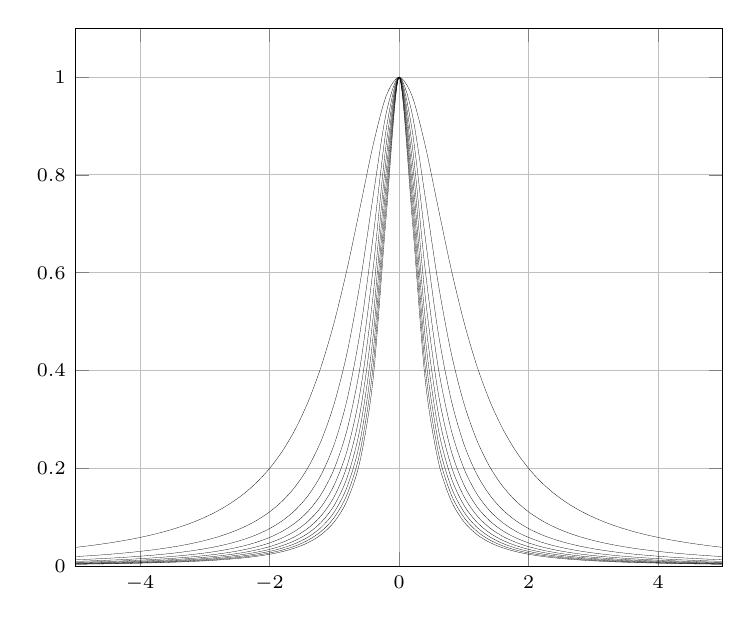
\begin{tikzpicture}
            \begin{axis}[domain=-5:5, restrict y to domain=0:1,
                xmin=-5, xmax=5, ymin=0, ymax=1.1, grid=both,
                tick label style={font=\scriptsize}, xscale=1.2, yscale=1.2]
                \addplot[samples=51,smooth,ultra thin] {1/(1 + 2*x^2)};
                \addplot[samples=51,smooth,ultra thin] {1/(1 + 3*x^2)};
                \addplot[samples=51,smooth,ultra thin] {1/(1 + 4*x^2)};
                \addplot[samples=51,smooth,ultra thin] {1/(1 + 1*x^2)};
                \addplot[samples=51,smooth,ultra thin] {1/(1 + 5*x^2)};
                \addplot[samples=51,smooth,ultra thin] {1/(1 + 6*x^2)};
                \addplot[samples=51,smooth,ultra thin] {1/(1 + 7*x^2)};
                \addplot[samples=51,smooth,ultra thin] {1/(1 + 8*x^2)};
                \addplot[samples=51,smooth,ultra thin] {1/(1 + 9*x^2)};
                \addplot[samples=51,smooth,ultra thin] {1/(1 + 10*x^2)};
            \end{axis}
        \end{tikzpicture}
    \end{figure}
\end{solution}

\subsection{Metryka Czebyszewa}
Weźmy pewną dwuargumentową funkcję zdefiniowąną jako
\[ d_c(f, g) = \sup_{x\in X}\left|f(x) - g(x)\right|. \]
Można udowodnić, że funkcja $d_c$ jest metryką (zwaną metryką Czebyszewa). Jako argumenty przyjmuje dwie funkcja zdefiniowane na tej samej dziedzinie $X$.

\begin{theorem}
    Jeśli każda funkcja ciągu funkcyjnego $(f_n(x))$ jest ograniczona, to
    \[ f_n \rightrightarrows f \Longleftrightarrow \lim_{n\lthen\infty}d_c(f_n, f) = 0 .\]
\end{theorem}

\begin{example}
    Zbadaj zbieżność punktową i jednostajną ciągu funkcyjnego
    \[ f_n(x) = \frac{x^n}{1 + x^n} \]
    na przedziale $[2, \infty)$.
\end{example}
\begin{solution}
    Mamy
    \[ \lim_{n\lthen\infty} \frac{x^n}{1 + x^n} = 1 \equiv f, \]
    więc ciąg jest zbieżny punktowo do funkcji ciągłej, możemy zatem sprawdzić, czy zbiega do niej jednostajnie.
    \[ \lim_{n\lthen\infty}\sup_{x\in X} \left|\frac{x^n}{1 + x^n} - 1\right| = \lim_{n\lthen\infty}\sup_{x\in X} \left(1 - \frac{x^n}{1 + x^n}\right)\]
    Obliczmy supremum danej funkcji.
    \[ \ddx \left(1 - \frac{x^n}{1 + x^n}\right) = \frac{nx^{n-1}(1 + x^n) - x^n(nx^{n-1})}{\left(1 + x^n\right)^2} = \frac{nx^{n-1}}{\left(1 + x^n\right)^2} \]
    Pochodna zawsze jest dodatnia, więc supremum będzie przy $x \lthen \infty$. Mamy
    \[ \lim_{n\lthen\infty}\sup_{x\in X} \left(1 - \frac{x^n}{1 + x^n}\right) = \lim_{n\lthen\infty}\lim_{x\lthen\infty} \left(1 - \frac{x^n}{1 + x^n}\right) = \lim_{n\lthen\infty} \left(1 - 1\right) = 0, \]
    więc dany ciąg jest zbieżny jednostajnie.
\end{solution}

\begin{example}
    Zbadaj zbieżność punktową i jednostajną ciągu funkcyjnego
    \[ f_n(x) = \frac{nx}{n^2 + x^2} \]
    na zbiorze $\RR$.
\end{example}
\begin{solution}
    Mamy
    \[ \lim_{n\lthen\infty} \frac{nx}{n^2 + x^2} = \lim_{n\lthen\infty} \frac{x}{n} = 0 \equiv 0, \]
    więc ciąg jest zbieżny punktowo do funkcji ciągłej, możemy zatem sprawdzić, czy zbiega do niej jednostajnie.
    \[ \lim_{n\lthen\infty}\sup_{x\in X} \left|\frac{nx}{n^2 + x^2}\right| = \lim_{n\lthen\infty}\sup_{x\in X} \left(\frac{nx}{n^2 + x^2}\right) \]
    Obliczmy supremum danej funkcji.
    \[ \ddx \left(\frac{nx}{n^2 + x^2}\right) = \frac{n(n^2 + x^2) - nx(2x)}{\left(n^2 + x^2\right)^2} = \frac{n^3 - nx^2}{\left(n^2 + x^2\right)^2} \]
    Pochodna zeruje się, gdy
    \[ n^3 = nx^2 \implies x = \pm n, \]
    więc supremum będzie przy $x = n$. Mamy
    \[ \lim_{n\lthen\infty}\frac{n^2}{n^2 + n^2} = \frac{1}{2}, \]
    więc dany ciąg nie jest zbieżny jednostajnie.
\end{solution}

\begin{theorem}[o różniczkowalności granicy ciągu funkcyjnego]
    \label{t:differentiable limit}
    Jeśli każda funkcja ciągu funkcyjnego $(f_n(x))$ jest różniczkowalna, ciąg $(f_n)$ jest zbieżny, a ciąg $(f_n')$ zbieżny jednostajnie, to dla każdego $x \in X$ zachodzi
    \[ \left(\lim_{n\lthen\infty} f_n(x)\right)' = \lim_{n\lthen\infty} \left(f_n'(x)\right). \]
\end{theorem}

\begin{theorem}[o całkowalności granicy ciągu funkcyjnego]
    \label{t:integrable limit}
    Jeśli każda funkcja ciągu funkcyjnego $(f_n(x))$ jest całkowalna, a ciąg $(f_n)$ jest zbieżny jednostajnie, to dla każdych $x_1, x_2 \in X$ zachodzi
    \[ \int_{x_1}^{x_2}\left(\lim_{n\lthen\infty} f_n(x)\right) \d x = \lim_{n\lthen\infty} \left(\int_{x_1}^{x_2} f_n(x) \d x\right). \]
\end{theorem}

    \section{Szeregi funkcyjne}
    Podobnie do szeregów liczbowych, szeregi funkcyjne to para $((f_n(x))_{n\in\NN}, (S_n(x))_{n\in\NN})$: ciąg funkcyjny oraz ciąg sum częściowych ciągu funkcyjnego. Taki szereg jest zbieżny (punktowo / jednostajnie) do sumy szeregu $S$, jeśli ciąg $(S_n(x))$ jest zbieżny (częściowo / jednostajnie) do $S$.

Analogicznie do twierdzenia \ref{t:uniform convergence implies pointwise convergence}, warukiem koniecznym zbieżności jednostajnej szeregu jest jego zbieżność punktowa.

Z kolei w analogii do twierdzenia \ref{t:necessary condition of convergence}, warunkiem koniecznym zbieżności (punktowej / jednostajnej) szeregu $\sum_{n=1}^\infty f_n(x)$ jest zbieżność (punktowa / jednostajna) ciągu funkcyjnego $(f_n(x))$ do zera, to znaczy
\[ \sum_{n=1}^\infty f_n(x) \rightarrow S \Longrightarrow f_n(x) \rightarrow 0 \equiv f \]
oraz
\[ \sum_{n=1}^\infty f_n(x) \rightrightarrows S \Longrightarrow f_n(x) \rightrightarrows 0 \equiv f. \]

\begin{theorem}[kryterium Weierstrassa]
    Jeśli istnieje taki ciąg $(a_n)$, że dla każdego $n \in \NN$ i dla każdego $x \in X \subset \RR$ mamy nierówność
    \[ |f_n(x)| \leq a_n \]
    oraz szereg $\sum_{n=1}^\infty a_n$ jest zbieżny, to szereg funkcyjny
    \[ \sum_{n=1}^\infty f_n(x) \]
    jest jednostajnie zbieżny na $X$.
\end{theorem}

Zachodzi twierdzenie o ciągłości, analogiczne do twierdzenia \ref{t:continuous limit}.

\begin{theorem}
    \label{t:continuous series}
    Jeśli szereg $\sum_{n=1}^\infty f_n(x)$ jest szeregiem funkcji ciągłych i jest jednostajnie zbieżny $\sum_{n=1}^\infty f_n(x) \rightrightarrows S(x)$, to funkcja $S$ jest ciągła.
\end{theorem}

\begin{example}
    Zbadaj zbieżność punktową i jednostajną szeregu
    \[ \sum_{n=1}^\infty x^n(1-x) \]
    na przedziale $[0,1]$.
\end{example}
\begin{solution}
    Dla $x \in [0, 1)$ mamy:
    \[ \sum_{n=1}^\infty x^n(1-x) = x(1-x)\frac{1}{1-x} = x, \]
    natomiast dla $x = 1$ mamy
    \[ \sum_{n=1}^\infty x^n(1-x) = \sum_{n=1}^\infty 1^n \cdot 0 = 0, \]
    więc szereg jest zbieżny punktowo. Funkcja
    \[ S(x) = \begin{cases}x, & \text{dla } x \in [0, 1) \\ 0, & \text{dla } x = 1 \end{cases}, \]
    do której dany szereg zbiega nie jest ciągła, a funkcje $f_n(x) = x^n(1-x)$ są ciągłe, więc, na mocy twierdzenia \ref{t:continuous series}, szereg nie zbiega jednostajnie.
\end{solution}

\begin{example}
    Zbadaj zbieżność punktową i jednostajną szeregu
    \[ \sum_{n=1}^\infty \frac{nx}{1+n^4x^2} \]
    na przedziale $[1,\infty)$.
\end{example}
\begin{solution}
    Dla każdego $x \in [1, \infty]$ oraz $n \in \NN$ mamy
    \[ \left|\frac{nx}{1+n^4x^2}\right| = \frac{nx}{1+n^4x^2} \leq \frac{nx}{n^4x^2} = \frac{1}{n^3x} \leq \frac{1}{n^3}, \]
    więc, na mocy kryterium Weierstrassa, dany szereg jest jednostajnie zbieżny, bo szereg harmoniczy rzędu $3$ jest zbieżny.
\end{solution}

\begin{example}
    Zbadaj obszar zbieżności\footnote{czyli zbiór punktów, w których szereg jest zbieżny} punktowej oraz zbieżność jednostajną szeregu
    \[ \sum_{n=1}^\infty \frac{x^2}{e^{nx}}. \]
\end{example}
\begin{solution}
    Możemy od razu stwierdzić, że dla $x = 0$ otrzymamy szereg ciąg zer, który oczywiście jest (jednostajnie) zbieżny do zera. Możemy potraktować $x$ jako parametr, wtedy zamiast szeregu funkcyjnego będziemy mieć szereg liczbowy, którego zbieżność możemy pokazać z kryterium d'Alemberta:
    \[ g = \lim_{n\lthen\infty} \frac{x^2}{e^{x(n+1)}}\frac{e^{xn}}{x^2} = \lim_{n\lthen\infty}\frac{1}{e^x} = \frac{1}{e^x}. \]
    Szereg jest więc zbieżny dla każdego $x > 0$ i rozbieżny dla każdego $x < 0$. Ostatecznie, obszar zbieżności punktowej danego szeregu funkcyjnego to $[0,\infty)$.

    Zajmijmy się teraz zbieżnością jednostajną. Oczywiście można by ją wykazywać przez znalezienie ciągu sum cześciowych, a następnie skorzystanie z twierdzenia \ref{t:uniform convergence iff metric = 0}, ale możemy też skorzystać z kryterium Weierstrassa, chociaż w dosyć nieoczywisty sposób.

    Znajdźmy najpierw supremum ciągu $a_n = \frac{x^2}{e^{nx}}$. Możemy znaleźć miejsca zerowe pochodnej:
    \[ \ddx \frac{x^2}{e^{nx}} = \frac{2x(e^{nx}) - x^2(ne^{nx})}{e^{2nx}} = \frac{x(2 - xn)}{e^{nx}} = 0 \iff x \in \left\{0, \frac{2}{n}\right\}. \]
    Szkicując wykres przekonamy się, że funkcja $a_n(x)$ osiąga maksimum w $x = \frac{2}{n}$, więc
    \[ a_n(x) \leq a_n\left(\tfrac{2}{n}\right) = \frac{\left(\frac{2}{n}\right)^2}{e^2} = \frac{4}{e^2n^2}. \]
    Szereg $\sum_{n=1}^\infty \frac{4}{e^2n^2}$ jest zbieżny (ponieważ jest harmoniczny rzędu $2$), więc możemy użyć kryterium Weierstrassa udowadniając, że dany szereg funkcyjny jest jednostajnie zbieżny.
\end{solution}

Zachodzą również twierdzenia o różniczkowalności i całkowalności, analogiczne do twierdzeń \ref{t:differentiable limit} i \ref{t:integrable limit}.

\begin{theorem}
    \label{t:differentiable series}
    Niech $(f_n(x))$ będzie ciągiem funkcji różniczkowalnych. Jeśli szereg $\sum_{n=1}^\infty f_n(x)$ jest zbieżny na $X$, a szereg $\sum_{n=1}^\infty f_n'(x)$ jest jednostajnie zbieżny na $X$, to dla każdego $x \in X$ zachodzi
    \[ \left(\sum_{n=1}^\infty f_n(x)\right)' = \sum_{n=1}^\infty f_n'(x). \]
\end{theorem}

\begin{theorem}
    \label{t:integrable series}
    Niech $(f_n(x))$ będzie ciągiem funkcji całkowalnych. Jeśli szereg $\sum_{n=1}^\infty f_n(x)$ jest jednostajnie zbieżny na $X$, to dla każdych $x_1, x_2 \in X$ zachodzi
    \[ \int_{x_1}^{x_2}\left(\sum_{n=1}^\infty f_n(x)\right)\d x = \sum_{n=1}^\infty \left(\int_{x_1}^{x_2}f_n(x)\d x\right). \]
\end{theorem}

\subsection{Szeregi potęgowe}
\begin{definition}
    \label{d:power series}
    Szereg potęgowy o środku w punkcie $c$ to szereg funkcyjny
    \[ \sum_{n=1}^\infty a_n(x - c)^n, \]
    gdzie $a_n, x, c \in \CC$.
\end{definition}

\begin{theorem}
    Jeśli szereg potęgowy
    \[ \sum_{n=1}^\infty a_n(x - c)^n \]
    jest zbieżny dla pewnego $x_1$, to jest zbieżny dla wszystkich $x_2$ takich, że
    \[ |x_2 - c| < |x_1 - c|, \]
    a jeśli nie jest zbieżny dla pewnego $x_1$, to nie jest zbieżny dla wszystkich $x_2$ takich, że
    \[ |x_2 - c| > |x_1 - c|. \]
\end{theorem}

Powyższe twierdzenie każe nam podzielić płaszczyznę zespoloną (względem danego szeregu potęgowego) na trzy rozłączne zbiory. Formalnie, jeśli weźmiemy
\[ r = \sup\left\{|x - c| : \text{ szereg } \sum_{n=1}^\infty a_n(x - c)^n \text{ jest zbieżny}\right\}, \]
to zbiór
\[ \{x \in \CC : |x - x_0| < r\} \]
nazwiemy \vocab{kołem zbieżności}. Dla wszystkich elementów z tego zbioru dany szereg jest zbieżny. Dla elementów na brzegu tego koła zbieżność jest nieokreślona, a dla elementów poza nim dany szereg nie jest zbieżny. Liczba $r$ to \vocab{promień zbieżności}. Dla $x=c$ dany szereg jest zbieżny.

\begin{remark*}
    Jeśli przyjmiemy w definicji szeregu potęgowego (\ref{d:power series}), że $a_n, x, c \in \RR$, to koło zbieżności staje się \vocab{przedziałem zbieżności}, a nieokreśloną zbieżność mamy tylko dla dwóch elementów: $c - r$ oraz $c + r$.
\end{remark*}

\vocab{Obszarem zbieżności} nazywamy zbiór będący sumą koła zbieżności oraz zbioru elementów z jego brzegu, dla których dany szereg potęgowy jest zbieżny.

\begin{theorem}[Cauchy'ego-Hadamarda]
    \label{t:Cauchy-Hadamard}
    Promień zbieżności jest dany jako
    \[ r = \frac{1}{\limsup\limits_{n\lthen\infty}\sqrt[n]{|a_n|}}, \]
    gdzie $r = \frac{1}{0}$ interpretujemy jako $r = \infty$, a $r = \frac{1}{\infty}$ jako $r = 0$.
\end{theorem}

Można podać dwa słabsze twierdzenia, które jednak często łatwiej jest stosować:
\[ r = \frac{1}{\lim\limits_{n\lthen\infty} \left|\frac{a_{n+1}}{a_n}\right|} \hspace{1em}\Longrightarrow\hspace{1em} r = \frac{1}{\lim\limits_{n\lthen\infty}\sqrt[n]{|a_n|}} \hspace{1em}\Longrightarrow\hspace{1em} (\ref{t:Cauchy-Hadamard}). \]

Mówimy, że ciąg (szereg) funkcyjny jest \vocab{niemal jednostajnie zbieżny} na przedziale $(a, b)$ jeśli jest jednostajnie zbieżny na każdym przedziale $[c, d] \in (a, b)$.

\begin{fact}
    Jeśli szereg potęgowy jest zbieżny w $(c-r, c+r)$, to jest bezwzględnie zbieżny w $(c-r, c+r)$ oraz niemal jednostajnie zbieżny w $(c-r, c+r)$.
\end{fact}

\begin{fact}
    Jeśli szereg potęgowy jest zbieżny w $(c-r, c+r)$ do $S(x)$, to funkcja $S(x)$ jest ciągła, różniczkowalna i całkowalna w $(c-r, c+r)$. Prawdziwe dla szeregów potęgowych są również tezy twierdzeń \ref{t:differentiable series} i \ref{t:integrable series}.
\end{fact}

\begin{theorem}[Abela]
    \label{t:Abel}
    Niech $\sum_{n=1}^\infty a_n(x - c)^n$ będzie szeregiem potęgowym zbieżnym do $S(x)$ o promieniu zbieżności równym $r$. Jeśli ten szereg jest zbieżny dla $x_1 = c - r$ oraz istnieje granica $\lim\limits_{x\lthen x_1^+}S(x)$, to
    \[ \lim_{x\lthen x_1^+}S(x) = S(x_1), \]
    czyli funkcja $S(x)$ jest prawostronnie ciągła w $x = c - r$. Analogicznie, jeśli szereg jest zbieżny dla $x_2 = c + r$ oraz istnieje granica $\lim\limits_{x\lthen x_2^-}S(x)$, to
    \[ \lim_{x\lthen x_2^-}S(x) = S(x_2), \]
    czyli funkcja $S(x)$ jest lewostronnie ciągła w $x = c + r$.
\end{theorem}

\begin{example}
    Znajdź sumę szeregu
    \[ \sum_{n=1}^\infty\frac{(n+1)(x+2)^n}{2^n} \]
    w każdym punkcie obszaru zbieżności.
\end{example}
\begin{solution}
    Stosując twierdzenie Cauchy'ego-Hadamarda (\ref{t:Cauchy-Hadamard}) możemy obliczyć promień zbieżności danego szeregu
    \[ r = \frac{1}{\lim\limits_{n\lthen\infty}\sqrt[n]{\frac{n+1}{2^n}}} = \frac{1}{\frac{1}{2}} = 2, \]
    tak więc przedział zbieżności to $(-4, 0)$.
    Dla $x = -4$ mamy
    \[ \sum_{n=1}^\infty\frac{(n+1)(-2)^n}{2^n} = \sum_{n=1}^\infty(-1)^n(n+1) \text{ -- rozbieżny, nie spełnia warunku koniecznego}, \]
    a dla $x = 0$
    \[ \sum_{n=1}^\infty\frac{(n+1)2^n}{2^n} = \sum_{n=1}(n+1) \text{ -- rozbieżny, nie spełnia warunku koniecznego}. \]
    Obszarem zbieżności jest więc przedział $(-4, 0)$. Policzmy teraz sumę. Dla każdego $x \in (-4, 0)$ mamy
    \begin{align*}
        S(x) &= \sum_{n=1}^\infty\frac{(n+1)(x+2)^n}{2^n} = \sum_{n=1}^\infty \left(\frac{(x+2)^{n+1}}{2^n}\right)' \overset{(\ref{t:differentiable series})}{=} \left(\sum_{n=1}^\infty\frac{(x+2)^{n+1}}{2^n}\right)' \\
        &= \left(\frac{(x+2)^2}{2}\frac{1}{1 - \frac{x+2}{2}}\right)' = \left(\frac{(x+2)^2}{-x}\right)' = \frac{2x(x+2) + (x+2)^2}{x^2} = \frac{4 - x^2}{x^2}.
    \end{align*}
\end{solution}

\begin{example}
    Znajdź sumę szeregu
    \[ \sum_{n=0}^\infty \frac{2^n(x - \frac{1}{2})^n}{n+1} \]
    w każdym punkcie obszaru zbieżności.
\end{example}
\begin{solution}
    Stosując twierdzenie Cauchy'ego-Hadamarda (\ref{t:Cauchy-Hadamard}) możemy obliczyć promień zbieżności danego szeregu
    \[ r = \frac{1}{\lim\limits_{n\lthen\infty}\sqrt[n]{\frac{2^n}{n+1}}} = \frac{1}{2}, \]
    tak więc przedział zbieżności to $(0, 1)$.
    Dla $x = 0$ mamy
    \[ \sum_{n=0}^\infty \frac{2^n\left(-\frac{1}{2}\right)^n}{n+1} = \sum_{n=0}^\infty \frac{(-1)^n}{n+1} \text{ -- zbieżny z kryterium Leibniza}, \]
    a dla $x = 1$
    \[ \sum_{n=0}^\infty \frac{2^n\left(\frac{1}{2}\right)^n}{n+1} = \sum_{n=0}^\infty \frac{1}{n+1} \text{ -- rozbieżny z kryterium ilorazowego}. \]
    Obszarem zbieżności jest więc przedział $[0, 1)$. Policzmy teraz sumę. Dla $x = \frac{1}{2}$ mamy
    \[ S(\tfrac{1}{2}) = \sum_{n=0}^\infty \frac{2^n0^n}{n+1} = 1 + 0 + 0 + \cdots = 1. \]
    Dla pozostałych $x$ zapiszemy
    \[ S(x) = \sum_{n=0}^\infty \frac{2^n(x - \frac{1}{2})^n}{n+1} = \frac{1}{x - \frac{1}{2}}\sum_{n=0}^\infty \frac{2^n(x - \frac{1}{2})^{n+1}}{n+1} = \frac{1}{x - \frac{1}{2}}\sum_{n=0}^\infty \int_{\frac{1}{2}}^x 2^n\left(t-\frac{1}{2}\right)^n\d t. \]
    Szeregi potęgowe są niemal jednostajnie zbieżne w swoim przedziale zbieżności, więc dla $x \in (0, 1)$ możemy zamienić znaki sumy i całki (twierdzenie \ref{t:integrable series})
    \begin{align*}
        S(x) &= \frac{1}{x - \frac{1}{2}}\int_{\frac{1}{2}}^x \sum_{n=0}^\infty 2^n\left(t-\frac{1}{2}\right)^n\d t = \frac{1}{x - \frac{1}{2}}\int_{\frac{1}{2}}^x \frac{1}{1 - 2(t - \frac{1}{2})}\d t \\
        &= \frac{1}{x - \frac{1}{2}}\int_{\frac{1}{2}}^x \frac{1}{2 - 2t}\d t = \frac{1}{x - \frac{1}{2}}\left[-\frac{1}{2}\ln(1 - t)\right]_{\frac{1}{2}}^x = \frac{1}{1 - 2x}\left(\ln(1 - x) - \ln{\frac{1}{2}}\right) \\
        &= \frac{\ln(2 - 2x)}{1 - 2x}.
    \end{align*}
    Z twierdzenia Abela (\ref{t:Abel}) wynika, że
    \[ S(0) = \lim_{x\lthen 0^+}\frac{\ln(2 - 2x)}{1 - 2x} = \ln(2), \]
    więc ostatecznie mamy
    \[ S(x) = \begin{cases}1, & \text{dla } x = \tfrac{1}{2} \\ \frac{\ln(2 - 2x)}{1 - 2x}, & \text{dla } x \in [0, 1)\setminus \{\tfrac{1}{2}\} \end{cases}. \]
\end{solution}

\begin{example}
    Znajdź sumę szeregu liczbowego
    \[ 1 - \frac{1}{3} + \frac{1}{5} - \frac{1}{7} + \ldots. \]
\end{example}
\begin{solution}
    Weźmy szereg funkcyjny
    \[ S(x) = \sum_{n=0}^\infty \frac{(-1)^n}{2n+1}x^{2n+1}. \]
    Wartość $S(1)$ jest szukaną sumą, jeśli tylko szereg jest zbieżny w tym punkcie. Niech $t = x^2$. Stosując twierdzenie Cauchy'ego-Hadamarda (\ref{t:Cauchy-Hadamard}) możemy obliczyć promień zbieżności szeregu:
    \[ r_t = \frac{1}{\lim\limits_{n\lthen\infty}\frac{2n+1}{2n+3}} = 1, \]
    tak więc szereg zbiega, gdy $t \in (-1, 1) \implies x \in (-1, 1)$. W punktach $x = -1$ i $x = 1$ szereg również jest zbieżny, co można pokazać z kryterium Lebniza.

    Policzmy teraz sumę (dla przedziału zbieżności $(-1, 1)$):
    \begin{align*}
        S(x) &= \sum_{n=0}^\infty \frac{(-1)^n}{2n+1}x^{2n+1} = \sum_{n=0}^\infty\int_0^x (-1)^n u^{2n} \d u = \int_0^x\sum_{n=0}^\infty (-1)^n u^{2n} \d u \\
        &= \int_0^x\sum_{n=0}^\infty (-u^2)^n \d u = \int_0^x \frac{1}{1 + u^2} \d u = \left[\arctan(u)\right]_0^x = \arctan(x).
    \end{align*}

    Skoro w $x = 1$ ten szereg też jest zbieżny, to z twierdzenia Abela (\ref{t:Abel}) mamy
    \[ S(1) = \lim_{x\lthen 1}\arctan(x) = \arctan(1) = \frac{\pi}{4}. \]
\end{solution}

    % \appendix
    % \section{Dodatek}
    % \begin{theorem}[Nierówność Bernoulliego]
    \label{t:Bernoulli's inequality}
    Jeżeli $x \geq -1$, to dla każdego $\alpha \geq 1$ zachodzi nierówność
    \[ (1 + x)^\alpha \geq 1 + \alpha x. \]
    Równość zachodzi wtedy i tylko wtedy, gdy $\alpha = 1$ lub $x = 0$.
\end{theorem}

\begin{theorem}[Nierówność między średnimi]
    \label{t:mean ineqality}
    \[ AM \geq GM \geq HM \]
\end{theorem}

\end{document}